\documentclass[]{project_report}
\usepackage{graphicx}
\usepackage{hyperref}
\usepackage{tikz}




%%%%%%%%%%%%%%%%%%%%%%
%%% Input project details
\def\studentname{Edward Instance}
\def\reportyear{2024}
\def\projecttitle{Advanced Web Development}
\def\supervisorname{Christos Dexiades}
\def\degree{BSc in Computer Science}
\def\fullOrHalfUnit{Full Unit} % indicate if you are doing the project as a Full Unit or Half Unit
\def\finalOrInterim{Project Plan} % indicate if this document is your Final Report or Interim Report

\begin{document}

\maketitle

%%%%%%%%%%%%%%%%%%%%%%
%%% Declaration

\chapter*{Declaration}

This report has been prepared on the basis of my own work. Where other published and unpublished source materials have been used, these have been acknowledged.

\vskip3em

Word Count: 

\vskip3em

Student Name: \studentname

\vskip3em

Date of Submission: 

\vskip3em

Signature:

\newpage

%%%%%%%%%%%%%%%%%%%%%%
%%% Table of Contents
\tableofcontents\pdfbookmark[0]{Table of Contents}{toc}\newpage

%%%%%%%%%%%%%%%%%%%%%%
%%% Your Abstract here
\chapter*{Abstract}
\addcontentsline{toc}{chapter}{Abstract}

Online shopping has become an integral part of everyday life, with over 50 million users in the UK this year alone. This number is projected to rise by more than 10 million in the next five years [1]. Most online stores charge transaction fees for sales made on their platforms. For example, Amazon profits from transactions between third-party sellers and users [2]. While these fees are lucrative for the platform, they significantly reduce profit margins for sellers, particularly small-scale vendors with already tight margins, making it potentially detrimental. In addition to transaction fees, most payment gateways charge interchange, scheme, and processing fees. Typically, companies integrate these costs into their pricing structure, passing the burden onto the end user to maintain profitability [3].

In response to this growing demand, this project aims to develop a full-stack web application that [briefly describe the purpose or unique value of your app], catering to both individual users and businesses.


\newpage

%%%%%%%%%%%%%%%%%%%%%%
%%% Introduction
\chapter{Timeline}


I plan to spend the beginning of term one working on my project plan and deciding on the technologies and frameworks that I will be using. Then I will start building my application, I will be focusing on the Web and Application tier's as the data model will be defined based on them. I am hoping to have an Minimum viable product (MVP) by the end of week 8 so that I have time to test it and create my interim report by the end of week 10. After the report is submitted and I have completed the presentation I am planning to re-evaluate my plan for term 2, I am also planning to do a review in week 6 to ensure that I am on track and to help me prioritise work.


 

\section{Term 1}


\begin{center}
    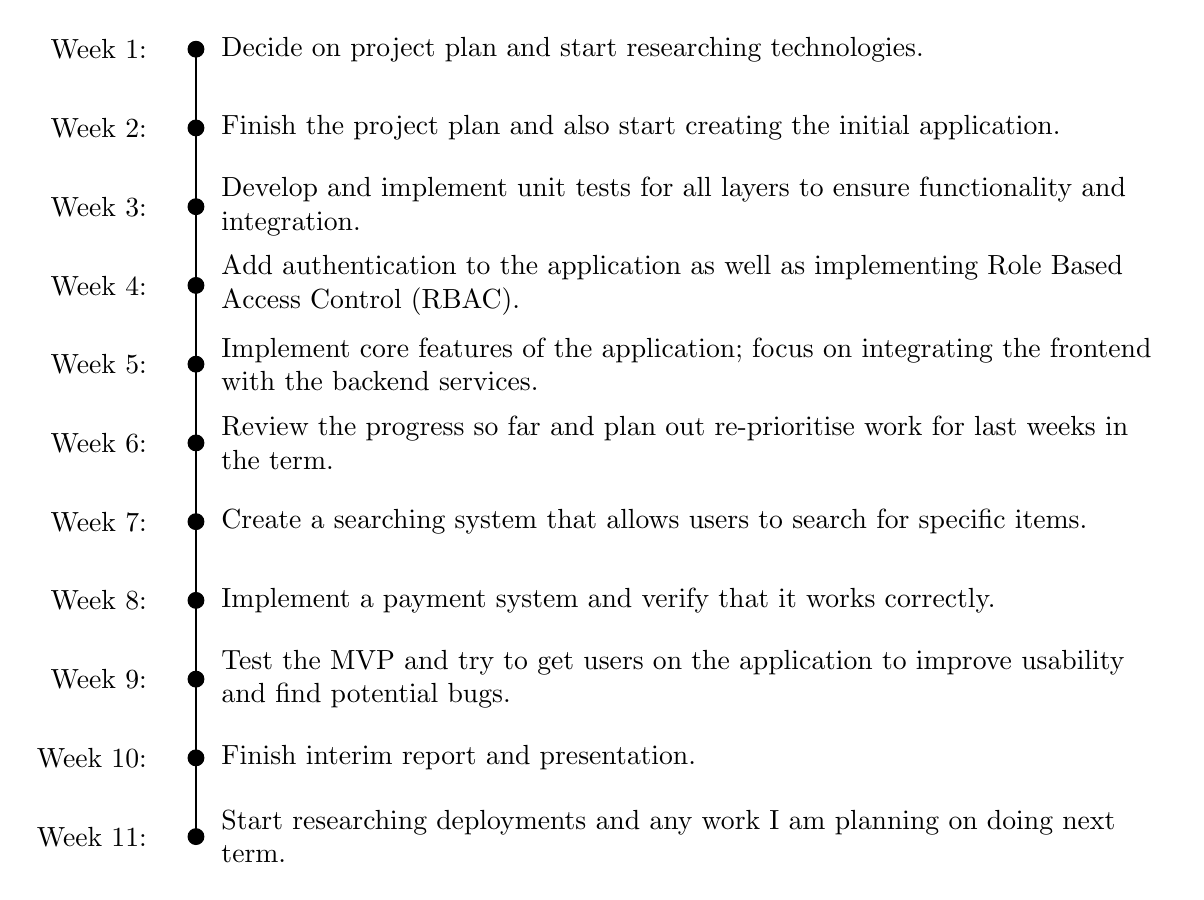
\begin{tikzpicture}[scale=1, every node/.style={scale=1}]

        \def\yshift{-1}  % Adjust the shift for better spacing
        % Draw the vertical timeline
        \draw[thick] (0,-1) -- (0,-11);  % Timeline from 0 to -10
        
        % Create the weeks and the dots for them
        \node[anchor=east] at (-0.5,\yshift) {Week 1:};
        \node[anchor=west, text width=12cm] at (0.2,\yshift) {Decide on project plan and start researching technologies.};
        \draw[fill] (0,\yshift) circle (0.1);  

        \node[anchor=east] at (-0.5,2*\yshift) {Week 2:};
        \node[anchor=west, text width=12cm] at (0.2,2*\yshift) {Finish the project plan and also start creating the initial application.};
        \draw[fill] (0,2*\yshift) circle (0.1);  

        \node[anchor=east] at (-0.5,3*\yshift) {Week 3:};
        \node[anchor=west, text width=12cm] at (0.2,3*\yshift) {Develop and implement unit tests for all layers to ensure functionality and integration.};
        \draw[fill] (0,3*\yshift) circle (0.1);  

        \node[anchor=east] at (-0.5,4*\yshift) {Week 4:};
        \node[anchor=west, text width=12cm] at (0.2,4*\yshift) {Add authentication to the application as well as implementing Role Based Access Control (RBAC).};
        \draw[fill] (0,4*\yshift) circle (0.1);  

        \node[anchor=east] at (-0.5,5*\yshift) {Week 5:};
        \node[anchor=west, text width=12cm] at (0.2,5*\yshift) {Implement core features of the application; focus on integrating the frontend with the backend services.};
        \draw[fill] (0,5*\yshift) circle (0.1);  

        \node[anchor=east] at (-0.5,6*\yshift) {Week 6:};
        \node[anchor=west, text width=12cm] at (0.2,6*\yshift) {Review the progress so far and plan out re-prioritise work for last weeks in the term.};
        \draw[fill] (0,6*\yshift) circle (0.1);  

        \node[anchor=east] at (-0.5,7*\yshift) {Week 7:};
        \node[anchor=west, text width=12cm] at (0.2,7*\yshift) {Create a searching system that allows users to search for specific items.};
        \draw[fill] (0,7*\yshift) circle (0.1);  

        \node[anchor=east] at (-0.5,8*\yshift) {Week 8:};
        \node[anchor=west, text width=12cm] at (0.2,8*\yshift) {Implement a payment system and verify that it works correctly.};
        \draw[fill] (0,8*\yshift) circle (0.1);  

        \node[anchor=east] at (-0.5,9*\yshift) {Week 9:};
        \node[anchor=west, text width=12cm] at (0.2,9*\yshift) {Test the MVP and try to get users on the application to improve usability and find potential bugs.};
        \draw[fill] (0,9*\yshift) circle (0.1);  

        \node[anchor=east] at (-0.5,10*\yshift) {Week 10:};
        \node[anchor=west, text width=12cm] at (0.2,10*\yshift) {Finish interim report and presentation.};
        \draw[fill] (0,10*\yshift) circle (0.1);  
        
        \node[anchor=east] at (-0.5,11*\yshift) {Week 11:};
        \node[anchor=west, text width=12cm] at (0.2,11*\yshift) {Start researching deployments and any work I am planning on doing next term.};
        \draw[fill] (0,11*\yshift) circle (0.1);  

    \end{tikzpicture}
\end{center}




\section{Term 2}

\chapter{Risks and Mitigation's}

\section{GDPR (General Data Protection Regulation) Concerns}

The risk here is failing to meet standards set by GDPR, failing to meet these standards can occur warnings, fines up to £20 million or 4\% of the business’s total annual worldwide turnover and potential bans on processing [4]. I have researched some of the main policies that an online shop should meet and how I plan to mitigate the overall risk of not meeting standards.

\subsection{Data Collection and Consent}
GDPR requires not only that data is only collected after obtaining consent from the user, but also that data is collected and used only for specific purposes, and must be deleted when those purpose are no longer applicable [5]. To ensure compliance, I will obtain explicit user consent before collecting personal data. This will be achieved through clear consent forms and notifications that have been based on the conditions for consent [6][Article 7 ] , this will ensure users understand how their data will be used.

\subsection{Data Minimisation}
“[Personal data shall be] adequate, relevant and limited to what is necessary in relation to the purposes for which they are processed [...]”[6] [Article 5, Sect. 1(c)]. Therefore only the necessary data for the service will be collected, the application will be designed to avoid unnecessary data collection in order to comply with the principle of data minimisation. I will also occasionally review what data I am collecting and if it is required.

\subsection{Data Security}
The controller and the processor shall implement appropriate technical and organisational measures to ensure a level of security appropriate to the risk[6] [Article 32, Sect. 1]. Some of the initial measures will be Data encryption both at rest and in transit will be implemented, but to ensure a good level of data security throughout the project I will also research and implement best practices.

\subsection{Data Retention}
Data should not be stored no longer than is necessary for the purposes for which the personal data are processed[6] [Article 5, Sect. 1(e)]. To mitigate this risk a clear data retention policy will be enforced, ensuring that personal data is not stored longer than necessary and data that is no longer needed will be securely deleted.

\subsection{User Rights}
Mechanisms will be in place to allow users to exercise their rights under GDPR which are listed here [6] [Chapter 3], including access to their data, the right to rectification, and the right to be forgotten.

\subsection{Third Parties}
Any third-party services used, such as payment gateways, authentication providers and more will be GDPR compliant. To ensure this I will look into documentation and check their policies.\newline



All of these GDPR policies affect the web application I will be building and the mitigation to them is to ensure that when any user data is being used or requested to make sure that it is for a reason, and to also have a 
plan on how to deal with data security and knowing what I might need to implement into the project as I have identified this risk.


\section{Security Risks}

There are many security risks when it comes to web applications and each of these require different solutions. My plan is to mitigate these vulnerabilities by focusing on the Open Worldwide Application Security Project (OWASP) Top Ten Web Application Security Risks [7]. This list highlights the most common and severe risks, which are frequently exploited by attackers, and thus have a high likelihood of being targeted. In addition to addressing these known vulnerabilities, I will continue to check for new risks as I progress.


\section{Scalability Issues}

As the application grows and creates a large user base there are issues related to scaling, if there are too many users for the application it could create unknown errors and potentially deny users access to the application. To mitigate this I plan to add load balancing and auto-scaling to the deployment steps, this should insure that the application will be able to handle increased and spiked traffic.

\section{Cost}

I am planing to either deploy this application on a server or by using a cloud provider and both of these solutions will incur costs. The main benefit to using a cloud provider is that it will trade the Capital Expense of setting up a server to Operational expenses, this can be a benefit as it means we do not need as much money to deploy the application but cloud computing costs can rapidly increase and go out of control. To mitigate this I am planning on setting up budget alarms and consistently monitoring the costs of the deployments so that it stays within a fixed budget I will decide on.

\section{User Authentication and Authorization Risks}

\section{Third-Party Dependencies}

\section{Cross-Browser Compatibility}

\section{Hardware Failure}

\section{Uneven Balance Between Report/Code}

\section{Over Optimistic Timeline}

%%%% ADD YOUR BIBLIOGRAPHY HERE
\newpage
\begin{thebibliography}{99}
\addcontentsline{toc}{chapter}{Bibliography}

\end{thebibliography}
\label{endpage}



\end{document}

